\chapter{Preparation}

In this chapter, I first develop the background of the computational problem of clustering 
directed graphs using spectral methods, by further explaining the well-studied methodology 
applicable to undirected graphs. Next, I introduce the two algorithms that have been developed to 
solve the problem, and describe how their respective methodologies contribute to this aim. 
Furthermore, I elaborate on the random-graph models that have been developed in conjunction with 
these algorithms, and how their usage for testing the algorithms is not entirely representative of 
real-world problems, which will help explain and justify the interest behind this project. Finally, 
I will discuss what requirements this project faced, as well as what the starting point for it 
was.

\section{Clustering}

This project concerns itself with one specific clustering problem. In general, however, clustering
is applicable to many more kinds of data than just graphs, for which many different algorithms have 
been developed to suit different needs. Perhaps the most common algorithm that clusters general, 
$m$-dimensional data is Lloyd's $k$-means clustering algorithm.

\subsection{$k$-Means Clustering}
Lloyd's $k$-means clustering algorithm is very widely used and fairly straightforward to 
understand. Given a set $D$ of points in $m$ dimensions, and an integer $k$, it returns the 
\emph{centroids} of $k$ clusters which partition $D$, such that the distances of points to their 
assigned centroids are locally minimised. It is presented in Algorithm \ref{algorithm:lloyd}.

It is, of course, important to note that the clusters returned by Lloyd's algorithm are only 
locally optimal. This, however, can be counteracted by running the algorithm several times with 
different initialisations of the centroids. Lloyd's algorithm operates on general data, and by 
terminating the algorithm at approximate, instead of absolute convergence or after a fixed number 
of iterations yields a reasonably fast run-time for the generally speaking NP-hard computational 
problem. 

\begin{algorithm}
\label{algorithm:lloyd}
	\caption{Lloyd's $k$-Means Clustering}

	\SetKwInOut{Require}{require}\SetKwInOut{Yield}{yield}
	\SetKwFunction{RandChoice}{random\_choice}
	\Require{Set $D$ of $m$-dimensional co\"ordinates, integer $k$}
	\Yield{Set $C$ of centroids of $k$ clusters underlying data in $D$.}
	\BlankLine
	\Begin{
		\tcp{Initialise centroids to arbitrary members of $D$}
		$C \longleftarrow$ \RandChoice$(k, D)$\;
		\While{set $C$ has not converged}{
			\tcp{Find data-centroid assignments}
			$\mathbb{C}\longleftarrow\{\mathbf{c}\mapsto\varnothing:\mathbf{c}\in C\}$\;
			\ForEach{$\mathbf{d} \in D$}{
				$\mathbf{c} \coloneqq \arg\min_{\mathbf{p}\in C}(\|\mathbf{p}-
				\mathbf{d}\|_2)$\;
				$\mathbb{C}(\mathbf{c})\longleftarrow \mathbb{C}(\mathbf{c}) \cup \{\mathbf{d}\}$\;
			}
			\tcp{Update positions of centroids to average of their respective clusters}
			$C \longleftarrow 
			\{\sum_{\mathbf{d}\in\mathbb{C}(\mathbf{c})}\mathbf{d} /|\mathbb{C}(\mathbf{c})|:\mathbf{c}\in C\}$\;
		}

		\KwRet{$C$}
	
	}
\end{algorithm}

These properties of Lloyd's algorithm mean that it would be convenient to use it as a basis for
algorithms clustering the vertices of a graph. To this end, one can consider a particular 
representation of an undirected graph known as its \emph{Laplacian}. 

\subsection{Spectral Methods}

\subsubsection{Undirected Graphs And Their Laplacians}
So, consider some undirected graph $G = (V, E)$ with adjacency matrix $A$. Suppose that $|V| = n$
such that $A$ is of dimension $n \times n$, and notice that $A$ is symmetric since $G$ is 
undirected. Now, consider the diagonal matrix $D$ that has $D_{i,i} = d_i$, where $d_i$ is the 
degree of vertex $i \in V$. Now, considering the construction 
$$
	\mathcal{L} \coloneqq D - A,
$$
the Laplacian of $G$, we note that $\mathcal{L}$ is still symmetric. This means that the 
eigenvalues associated to its eigenvectors are all real. Indeed, suppose that $G$ is disconnected
with $k$ connected components. Then consider, for any one (say $G_1$) of these connected components
the vector $e$ defined by $e_i = 1[i \in G_1]$. Then we have 
\begin{align*}
	(\mathcal{L} \times e)_i &= (D \times e)_i -(A \times e)_i \\
	&= d_i e_i - \sum_{v \in V} A_{i,v} \cdot e_v \\
	&= d_i 1[i \in G_1] - \sum_{v\in V} 1[i \leadsto v] \cdot 1[v\in G_1]
\end{align*}
where the first term will either be zero, should $i\notin G_1$, or the degree of $i$ otherwise. 
The second term will also be zero when $i \notin G_1$, since $i\leadsto v$ and $i \notin G_1$ imply
$v \notin G_1$, i.e.\ $1[v \in G_1] = 0$. Otherwise, the summand in the second term will be 1 
whenever $i \leadsto v$, that is, the second term will be $d_i$. Thus, $\mathcal{L}\times e = 
\mathbf{0}$, the zero vector. In other words, the vector $e$ is an eigenvector of $\mathcal{L}$ 
with eigenvalue 0, and since such a vector can be defined for each connected component of $G$, the
algebra\"ic multiplicity of $0$ in the characteristic polynomial of $\mathcal{L}$ is equal to the 
number of connected components in $G$\footnote{Strictly speaking this finds a lower bound on the 
number of eigenvectors with eigenvalue 0, but establishing the same upper bound is not difficult.}.

\subsubsection{Spectral Clustering}
In the setting of undirected graphs, the notion of similarity between two graph vertices is roughly 
equivalent to the question of how well-connected the vertices are. In the extreme, consider the case
where we wish to find $k$ clusters of graph nodes, and suppose again that the graph happens to have 
exactly $k$ connected components. Then, with our notion of vertex similarity, the $k$ clusters 
found by a reasonable algorithm should return the connected components of the graph. Therefore, 
consider the eigenpairs $(\lambda_i, e_i)$ of the Laplacian in this scenario, where $|\lambda_1| 
\leq |\lambda_2| \leq \hdots \leq |\lambda_n|$. We know that $\forall 1\leq i \leq k$, $\lambda_i 
=0$ and for all other $i$, $\lambda_i \neq 0$. Hence, by choosing the eigenvectors corresponeding
to the lowest $k$ eigenvalues, consider the $n$ $k$-dimensional points $p_1 \hdots p_n$ obtained by
setting $(p_j)_i = (e_i)_j$. These points will form the $k$ canonical basis vectors for $k$ 
dimensions, for any two vertices $u,v$ in the same connected component of $G$ will lie on the same 
point, meaning that Lloyd's algorithm will clearly quickly recover the connected components very 
quickly.

In the more general setting where the number of connected components is lower than the number of 
desired clusters (and, most commonly, where the graph is connected), intuitively it could be 
argued that this method would not work. However, it should be noted that Davis and Kahan 
established in 1969 that modifying a matrix insignifcantly does not perturb the space spanned by 
its eigenvectors significantly. This has the following significance for graph clustering: If we 
consider any graph to have an underlying, disconnected graph with $k$ connected compoonents, which
has been modified by adding (or perhaps removing) noisy edges, then the original disconnected graph
(which we can take to be our desired clustering) can be recovered by applying the method described 
above to the Laplacian of the noisy graph (that is, by considering the bottom $k$ eigenvectors, 
ordered by eigenvalue magnitude).

This method is known as the \emph{spectral clustering} algorithm for graphs (the relevant etymon 
being the \emph{spectrum} of the Laplacian). It works because the Laplacian captures the important 
information about node connectivity, and so do its eigenvectors. However, it relies on the fact that
the eigenvalues of the laplacian are real, which was guaranteed by the fact that the Laplacian is 
symmetric. This foreshadows one of the difficulties with spectral clustering methods for directed 
graphs, the adjacency matrices of which are not symmetric.

\subsection{Directional Communities and Clustering}

Besides the difficulty mentioned above, the problem of clustering directed graphs according to 
vertex similarity suffers another impairment: The notion of what made vertices of undirected 
graphs was simple enough, and made for an easy way of representing the graph in a format amenable 
to Lloyd's algorithm. However, since directed graphs have no equivalent notion of connectivity, 
this notion can no longer be used in this setting. This raises the question of how one should 
think about communities in directed graphs. 

\subsubsection{Directional Communities}
A first, simplistic, approach to remedying these issues is to remove the directional information 
from the graph and proceed by clustering it exactly as before. However, this misses the point of 
the task at hand. Consider, for example, a network that represents global trade. By removing the 
information of what directions goods flow in, we could not obtain clusters that take into account 
exporting and importing nations, attributes which should be of particular interest when  
considering what makes different countries similar with respect to trade. 

Instead of the extent of connectedness between two groups of vertices, therefore, a notion of 
`directional communities' emerged, in which the interactions between nodes of different 
commmunities became important, rather than the interactions of nodes within one cluster. 
This is particularly interesting when considering bipartite graphs. Consider for example a data 
set detailing the membership of a set of words in a set of texts, and the graph representing this 
membership relation. One can measure the similarity of texts by the words they contain, or the 
similarity of words by the texts in which they occur. Thus clustering the graphs by keeping in 
mind the sending and receiving behaviours of nodes allows for helpful insights in machine learning. 

\subsubsection{The DiSim Algorithm}
This project considers two main algorithms that have been developed to deal with such directional 
communities. The first of these was developed by Rohe et al.\ ; called DiSim. It is a fairly light 
modification of the classical spectral clustering algorithm, in tterms of the constructions it 
uses to cluster the graph. 

The algorithm first construct a so-called `regularized graph Laplacian', which, given the 
adjacency matrix $A$, defined as 
$$
	L \coloneqq O^{-\sfrac{1}{2}}\times A\times P^{-\sfrac{1}{2}} 
$$
where $O$ and $P$ are diagonal matrices storing each node's out- and in-degree respectively, 
offset with a parameter $\tau$ that defaults to the average out-degree. From this construction, it 
computes, instead of the eigenvectors of this Laplacian (which would not correspond to real 
eigenvalues, and so could not be ordered), the left and right \emph{singular} vectors which record 
the sending and receiving behaviours of the graph's nodes, respectively. 

The singular vectors correspond to singular values which behave analogously to the eigenvalues 
from before, but in DiSim, the `top' singular vectors are selected to base a clustering upon. 
This is because of the slightly differeent construction of $L$ in this case than $\mathcal{L}$ 
before. Another modification this algorithm makes is that it allows its user to cluster directed 
graphs particular with respect to `sending' or `receiving communities' in the case of bipartite 
graphs such as the word-text-membership example from before. 

However, when the graph is not bipartite, the algorithm can be modified only slightly to produce a 
clustering that takes into account both sending and receiving patterns by combining the right and 
the left singular vectors. It is this use case that this project focusses on in particular, since 
it allows for direct comparison to another algorithm developed exclusively for that purpose by
Cucuringu et al. 

\subsubsection{Hermitian Spectral Clustering}
In the development of this next algorithm (which I shall call Herm), another approach was taken 
that actually preserves the 
benefit of having real eigenvalues to work with. This approach was to represent the graph, instead 
of by a real adjacency matrix, by a complex-valued one. It is presented in Algorithm 
\ref{algorithm:herm}. This approach allows the preservation of the directional information whilst 
also retaining a simple representation of the graph. 
\begin{algorithm}
	\caption{Hermitian Spectral Clustering (Herm) \label{algorithm:herm}}
	\SetKwInOut{Require}{require}\SetKwInOut{Yield}{yield}
	\Require{Adjacency Matrix $A$ of graph $G$, integer $k$, $\epsilon \in \mathbb{R}^+$}
	\Yield{Partition of $G$ into directional communities}
	\BlankLine
	\tcp{Compute Hermitian representation of $G$}
	$A_\mathrm{Herm} \coloneqq \imath \cdot A - \imath\cdot A^T$\;
	$\{(\lambda_i, e_i)\} \longleftarrow$\ those eigenpairs of $A_\mathrm{Herm}$ such that 
	$|\lambda_i| > \epsilon$\;
	\tcp{Eigenvectors are complex, however, so represent graph as real data}
	$P \longleftarrow \sum_i e_i \times e_i^H$\;
	\KwRet{Result of applying Lloyd's algorithm to the rows of $P$, with $k$ clusters}
\end{algorithm}

A few comments: Here, $\imath$ denotes the imaginary unit; $\imath \coloneqq \sqrt{-1}$. Given a 
matrix $X$, its transpose is denoted $X^T$ and its conjugate transpose $X^H$. Lastly, the matrix $P
$ that is constructed as part of the algorithm is actually real, which is guaranteed by properties 
of $A_\mathrm{Herm}$ that are not essential to understanding the algorithm.

To get a better understanding of why this works, consider an alternative definition of 
$A_\mathrm{Herm}$:
$$
	(A_\mathrm{Herm})_{i,j} \coloneqq
	\begin{dcases}
		\imath & i \leadsto j \\
		- \imath & j \leadsto i \\
		0 & \text{otherwise.}
	\end{dcases}
$$
Therefore, $A_\mathrm{Herm}^2$ can be written as follows:
\begin{align*}
	(A_{\mathrm{Herm}}^2)_{i,j} &= \sum_{l} A_{i,l} \cdot A_{l, j} \\
	&=\sum_l \imath \cdot (1[i \leadsto l] - 1[l \leadsto i]) \cdot \imath \cdot 
	(1[l \leadsto j] - 1[j \leadsto l]) \\
	&= \sum_l (1[i \leadsto l]\cdot1[j \leadsto l] + 1[l \leadsto i]\cdot1[l 
	\leadsto j]) - \sum_l (1[i \leadsto l]\cdot1[l \leadsto j] + 1[l \leadsto i]\cdot1[j 
	\leadsto l])
\end{align*}
which means that the matrix $A_\mathrm{Herm}^2$ counts the number of nodes that are either common 
parents or common children of $i$ and $j$ whilst discounting nodes that have differently oriented 
connections to $i$ and $j$, respectively. Since $A_\mathrm{Herm}$ has the same eigenvectors as 
$A_\mathrm{Herm}^2$, $A_\mathrm{Herm}$ also implicitly tracks this. This is why taking the top 
eigenvectors of this matrix is the right choice, as opposed to the bottom eigenvectors as used in 
the typical spectral clustering algorithm. 

To provide a baseline to compare these algorithms against, one can consider basic modifications
to the graph's adjacency matrix $A$ which explicitly track the qualities of a graph in a similar 
way as $A_\mathrm{Herm}$ such as the matrices
\begin{itemize}
	\item $A^T \times A$, which tracks the number of common parents of nodes $i, j$,
	\item $A \times A^T$, which tracks the number of common children of nodes $i,j$ or
	\item their sum, which tracks both, very similarly to the matrix $A_\mathrm{Herm}$. However, 
	it should be noted that it does not penalise nodes with opposite sending/receiving 
	connections to $i,j$ respectively, and is much more expensive to calculate since matrix 
	multiplication is required.
\end{itemize}

\section{Supporting Graph Models}

In the development of the algorithms presented above, both teams of researchers developed models of
random graphs that exhibit directional communities; the purpose of this was to able to evaluate 
the performance of their algorithms aginst a known ground truth. Therefore, let me remind the reader
of two basic random-graph models that underly those models.

\subsection{Undirected Random Graphs}

Recall perhaps the most basic model of random graph, the Erd\H{o}s-R\'enyi model $\mathcal{G}(n,p)$ 
taking parameters $n \in \mathbb{N}$ and $p \in [0, 1]$. In a graph $G \sim \mathcal{G}(n,p)$, 
$V(G) = [n]$, and two nodes $i,j$ are connected in $G$ with probability $p$.

A slightly more advanced random-graph-model is the so-called Stochastic Block-Model (SBM). Given
parameters $k, n \in \mathbb{N}$, $p, q \in [0,1]$, a graph sampled from the SBM has $k \cdot n$
nodes, separated in $k$ clusters of $n$ nodes each. Within a cluster, two nodes are connected with
probability $p$, when nodes $i, j$ are in separate clusters, they are connected with probability 
$q$. Of course, a slight (but not very interesting) variation of this model would allow for 
heterogeneous cluster sizes. 

\subsection{Directed Communities With a Directed SBM}

To suppert the evaluation of Herm, Cucuringu et al.\ proposed a \emph{directed} stochastic 
block-model (DSBM). This model is naturally based on the SBM of before, but adds a parameter $\mathcal{F}
\in [k] \times [k] \rightarrow [0,1]$. Let us consider this parameter as a matrix storing, for each
ordered pair $(c_1, c_2)$ of clusters, the probability of an edge between the two clusters being 
oriented from $c_1$ to $c_2$. Notice that therefore, $\mathcal{F}_{i,j} = 1-\mathcal{F}_{j,i}$, and
so $\mathcal{F}_{i,i} = \sfrac{1}{2}$ for any $i$.

The DSBM behaves just like the previous SBM, but then orients all edges in the resulting graph 
according to $\mathcal{F}$. This means that the nature of directional relationships in the graph
is easily configurable by changing the parameter $\mathcal{F}$. To make this clearer, consider the 
example as presented below.

Consider a graph that models information flow between four clusters of vertices, and suppose that
there are two source clusters, one intermediate cluster and one final cluster of vertices that 
gather information, collate information and process information, respectively. Then the nature of 
communication between clusters would necessarily have to model a progressive movement of 
information, i.e.\ all communication would have to majoritatively flow from `earlier' to `later' 
clusters. Figure \ref{figure:infoflow} presents the meta-graph of a possible such network and the 
directions of communication. 
\begin{figure}
	\begin{center}
	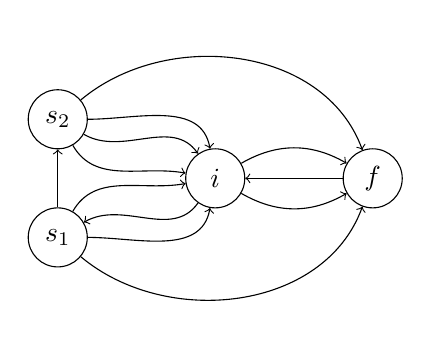
\begin{tikzpicture}
		\node[draw, circle, minimum size=0.75cm] (s1) at (0,0) {$s_1$} ;
		\node[draw, circle, minimum size=0.75cm] (s2) at (0,1.5) {$s_2$} ;
		\node[draw, circle, minimum size=0.75cm] (i) at (2,0.75) {$i$} ;
		\node[draw, circle, minimum size=0.75cm] (f) at (4,0.75) {$f$} ;
		\draw[->] (s1) edge[out=60, in=190] (i); 
		\draw[->] (s1) edge[out=0, in=260] (i); 
		\draw[->] (i) edge[out=235, in=30] (s1);
		\draw[->] (s2) edge[out=-60, in=-190] (i); 
		\draw[->] (s2) edge[out=0, in=-260] (i); 
		\draw[->] (s2) edge[out=-30, in=-235] (i);
		\draw[->] (s1) edge[out=90, in=270] (s2);
		\draw[->] (i) edge[out=30, in=150] (f);
		\draw[->] (i) edge[out=-30, in=-150] (f);
		\draw[->] (f) edge[out=180, in=0] (i);
		\draw[->] (s1) edge[out=-40, in=-110] (f); 
		\draw[->] (s2) edge[out=40, in=110] (f); 
	\end{tikzpicture}
	\end{center}
	\caption{The meta-graph of a network modelling information flow, comprising source clusters
	$s_1, s_2$, intermediate cluster $i$ and final cluster $f$.}
	\label{figure:infoflow}
\end{figure}
Such a communications network could then be modelled by an $\mathcal{F}$ such as the following:
$$
	\mathcal{F} = 
	\begin{pmatrix}
		\sfrac{1}{2} & 1 & \sfrac{2}{3} & 1 \\
		0 & \sfrac{1}{2} & 1 & 1 \\
		\sfrac{1}{3} & 0 & \sfrac{1}{2} & \sfrac{2}{3} \\
		0 & 0 & \sfrac{1}{3} & \sfrac{1}{2} \\
	\end{pmatrix}
$$

The advantage of this model is that it is easily understood and configurable, since only one 
parameter needs to be tuned to give such graphs meaning in the sense we might care about. However, 
we should also note its disadvantages: Firstly, it does not allow for varying quantities of 
communication between clusters; between any two clusters, the number of edges concentrates around 
$qn^2$. Secondly, the degrees of all vertices in the graph are highly homogeneous; with high 
probability, each node has degree (in the undirected projection of the graph) approximately $pn + 
(k-1) q n$. 

While a so-called Stochastic co-BM (ScBM) developed in support of DiSim can be modified to address 
the second issue, the first issue remains even there; that model is a generalisation of the DSB, 
the main advantage of which is that it allows for bipartite graphs which is not of particular 
interest for this project. Furthermore, the way to address the homogeneous degree distribution 
here is complicated and requires a fixxing the in- and out-degrees of each indivdual vertex, which 
makes working with these `degree-corrected' ScBM graphs. 

\subsection{Real-World Graphs}
This difficulty is significant. This is because many interesting networks in real-life settings 
follow very heterogeneous degree distributions: To return to our previous example, word frequencies
are distributed according to a Zipf distributions in most natural languages, which exhibit very 
long power-tails. Another source of examples for such power-tail distributions is the setting of 
research papers; graphs that are formed by adding edges representing citations between to papers 
(so-called citation networks) have also been shown to follow power-tail distributions of vertex 
degrees. 

Indeed, many such networks that grow over time do, including the internet. To model their growth, 
Price developed a random-graph model that utilises a technique known as preferential attachment. 
In this model, the sampled graph grows over time, adding one node at a time which forms edges 
according to some specified distributions, where each edge attaches more probably to vertices that
already have many incoming edges. This graph model is supported by a smoothing parameter $a$ that 
ensures that new vertices can also gain citations, which can be adapted to fit empirically determined
values.

\section{Requirements Analysis}

\subsubsection{Motivations}
It is one aim of this project to evaluate the performace of the existing algorithms on graphs 
that exhibit such power-tail distributions since little research in this are has so far been done
concerning the detection of directional communities and the algorithms have mainly been applied to 
graphs that were constructed according to models that would naturally approximte idealised inputs.
This means that there is scientific interest in the renewed evaluation of the algorithms outside of
the control of their respective developers, while also expanding on the experiments done previously.

\subsubsection{Generating Irregular Graphs}
To this end, it will be necessary to be able to produce graphs efficiently which exhibit both a 
degree distribution mirroring that of real-world graphs, since the interest in this project lies 
with the applicability to real-world machine-learning challenges, whilst also exhibiting the kind 
of directional communities that define the DSBM. That is, these graphs need to have some known
ground truth about the community structure that expresses itself in the interactions between 
communities. Furthermore, controlling these directional communities should remain easily 
understandable in order to make this study and evaluation of the algorithms reproducible and 
adaptable for new purposes. 

This means that a random model for the generation of such graphs needs to be developed, drawing on
the graph models that already exist to provide a basis for comparison. This model should remain 
understandable and not overly complex to sample from, since the graphs used are not in the focus of
this project. Furthermore, it should be possible to generate these graphs \emph{efficiently} so as
not to slow down the evaluation process drastically.

\subsubsection{Algorithm Performance}
It is besides the interest of this project to analyse how efficiently the algorithms operate, since
the algorithms are formulated from a very high level, so by using partwise solutions to the 
indivdual steps that are as efficient as possible, the algorithms' efficiency may be optimised. 
It is more of interest to determine the quality of any output produced, to which end a performance
criterion needs to be selected and its measurement efficiently implemented. Nevertheless, in the case
that the graphs grow large, since the representaion of the graphs is in matrix form, all steps of the
process will need to utilise quick linear-algebra implementations in order to make testing viable.

It will also be relevant to provide a comparison in performance between operating on graphs sampled
from the heterogeneous model and graphs sampled from the previous models; since the graph models
developed earlier are very suitable for the respective algorithms, the performance on those graphs
will provide an upper bound for the optimal performance of the clustering algorithms. Therefore, 
a correspondence between the previous graph models and the one developed as part of this project 
is required.

\subsubsection{Improving Performance}
In the setting of undirected graphs, modifications to the input graphs have been made to improve the
performance of spectral clustering methods. After obtaining results for the clustering performance 
on the irregular graphs, it will be interesting to evaluate these techniques' applicability to 
the setting of clustering directed graphs with the purpose of recovering directional communities.

\subsubsection{Scientific Validity}
Throughout the experimentation process in this project, the previously conducted experiments are
considered in order to guide which dimensions are explored, and in what sense those experiments can
be expanded upon. All decisions in the evaluation process have to be guided by a correspondence to
the real world to justify the effort invested and the interest in this poject. This means drawing 
on both shortcomings of previous research, as well as using past techniques and existing ideas to
improve the scientific integrity of the project.

Another factor in ensuring the scientific validity of this project will be to ensure statistical 
significance of the performance results, since the experimentation graphs are largely random. This,
however, will not be difficult to ensure with sufficiently large graphs and multiple experiments 
using different graphs sampled from the same distribution.

\section{Starting Point}
The concepts of graph clustering and random (as well as real-world) graphs were briefly 
introduced in the Paper 3 course \emph{Machine Learning and Real-world Data}. In that 
course, however, the problem was approached programmatically where my project will employ 
spectral methods. The linear algebra thus required for the project was touched on in the 
course \emph{Mathematical Methods I} from the Natural Sciences Tripos, and linear algebra 
in general is used in a number of courses of Part I of the Computer Science Tripos. 
\par
In the specific area of spectral clustering, there have been a few research papers 
concerning the detection of `directional' communities, introducing models of random 
digraphs with community structures, which should help extend undirected random graph models for this project. 
The project will involve implementing and refining algorithms presented in previous research. 
Furthermore, there is some pre\"existing literature on regularising undirected graphs for 
the purpose of clustering, 
from which I will draw a starting point for the corresponding 
parts of the project.

